%!TEX root = monsterhunter.tex
\renewcommand*{\hbPartCover}{assets/ext/world-cover}
\renewcommand*{\hbPartSubcover}{assets/ext/world-cover2}

\part{Exploring the World}

\chapter{Geography}

\hbWideBottomArtFirstPage{1.784}{.892}{assets/ext/fields-of-gold}

Though population is sparse, life flourishes in every corner of the world. People have constructed impressive cities despite the constant threat of monster attack everywhere from the scorching desert to freezing mountaintops. And in between the buildings of the modern civilisation we can find the ruins of those who came before us, a mysterious society only known as the Ancient Civilisation.

\section{Regions}
We are not given an estimate of the size of the Monster Hunter World. The size of the world is an important customisation factor. We know that the Hunter's Guild is a single global organisation. While its administration is decentralised this still implies that one can travel from one end to the continent in reasonable time. But how long is reasonable? Without a forced march, characters can travel 30 miles per day at fast pace (a reckless act considering how dangerous the world is). These are various options for the size of your world:

\paragraph{Small} Minegarde and Dundorma are about 600 miles apart, or 20 days of travel (about the distance of Berlin to Paris). That puts the total coast to coast distance of the continent to about 1500 miles or 50 days of travel.

\paragraph{Medium} Minegarde and Dundorma are about 1500 miles apart (about the distance between London and Moscow). The whole continent is 3800 miles (about 130 days of travel) east to west.

\paragraph{Large} The continents on the map, which somewhat resemble Europe, Asia and Africa are about the same size as those real-life continents. That means the width of the main continent are about 6000 miles, or 200 days of fast travel pace. Dundorma and Minegarde are about 2400 miles apart.

\hbWideBottomArtFirstPageFix

\begin{hbNoteWide2}[b]
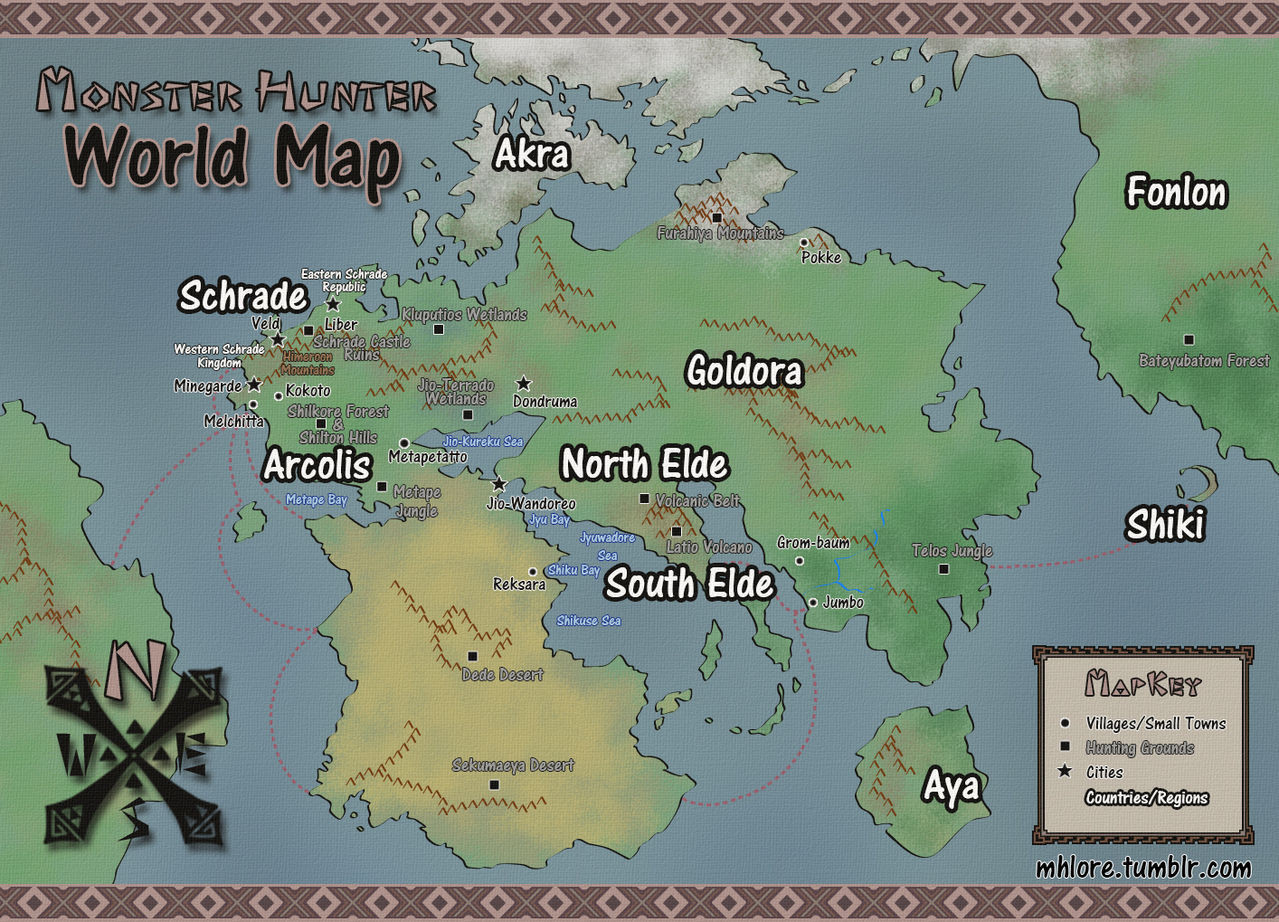
\includegraphics[width=\textwidth]{assets/ext/MHMap.jpg}
\end{hbNoteWide2}

\subsection*{Schrade}
This region was split in two by a civil war long ago, and is now divided into the Western Schrade Kingdom and the Eastern Schrade Republic, with the ancient ruins of Castle Schrade positioned roughly in the middle.

\paragraph{Liber} The capital of the Eastern Schrade Republic. Situated in a basin surrounded by steep mountains, it is subjected to severe weather and long winters. It is a prosperous and egalitarian trade city, famous for its monster hunting caravans. The center of town is dominated by a heavily fortified tower for monitoring and repelling large monsters.

\paragraph{Veld} The capital of the Western Schrade Kingdom. A walled fortress city of opulent aristocrats. The poor are relegated to slums outside the city walls, an area sarcastically named "The Painting District".

\paragraph{Castle Schrade} An ancient castle located in the vast open plain in the center of Schrade. Once a splendid feudal manor, it is now a mere shadow of its former glory, surrounded only by the ruins of the villages and towns that used to encircle it. So complete is the devastation, that no one remains to mourn its passing.

\paragraph{Kokoto Village} A small town of subsistence farmers in a forested area with a mild climate. The village relies on its chief and his deep understanding of monsters and monster ecology to maintain a peaceful relationship with nearby monsters, however, hunters are still needed on occasion to defend the town.

\paragraph{Minegarde} The city of Minegarde is an outpost built on a small outcropping with several caves among the rocky cliffs.  It was found to be rather unsuitable for usual human habitation due to the arid, rocky location and large amounts of dangerous monsters, so it became a haven for hunters and those that do business with them.  Because of the monsters, Minegarde also has multiple cannons for defense.  The cave that the blacksmith is located in is used as an emergency shelter for the locals should monsters attack.  The blacksmiths of Minegarde are also responsible for creating the first prototypes for the Gunlance.

\subsection*{Arcolis}
\paragraph{Melchitta} Melchitta is a rather new village situated on the shore of The Great Circle Lake, a lake that was formed by a meteor strike. It was originally just a tiny hunting village until some scholars from Minegarde took note of it, and now trade is booming.

\paragraph{Loc Lac} Loc Lac is a large, prosperous desert city built at the edge of the sand sea, near a large lake. The lake was formed when Jhen Mohran crashed into the rocks and its tusk lodged into the earth so deeply it struck water. The people of Loc Lac consider Jhen to be a symbol of prosperity, because the creation of the lake allowed the city to flourish. They hold the "Festival of Fear" every time the sandstorms arrive that herald Jhen's approach.

\subsection*{Akra}
Far to the North is the freezing, ice-covered Akra Region, known for its volatile weather. Despite the harsh conditions, it is surprisingly well populated. However, no major cities are located there.

\subsection*{Aya}
Far to the south is the island nation of Aya. It boasts a multitude of extremely varied tribal cultures, which a single absolute monarchy has (attempted) to rule over for generations.  Although most of the land's cultures are extremely isolationist, even those that aren't are still shrouded in mystery.

\subsection*{Fonlon}
\paragraph{Bateyubatom Forest} Also known as the Great Forest or the Everwood, this forest is home to a great variety of monsters and was also a major site of the old civilisation, as evidenced by the many ruins found scattered around the region.

\subsection*{Dundorma} Dundorma is located smack in the middle of the main continent, just on the other side of the Himeroon mountains. Due to its location it is constantly under threat from monsters, especially Elder Dragons. Despite having been destroyed repeatedly, it is always rebuilt and reinforced. As a result, its population fluctuates somewhat, but it is considered the largest city in the world with about 20,000 inhabitants. Dundorma is the seat of the Hunter's Guild administration, as well as the home of His Immenseness, the Great elder of Dundorma, a wise old wyverian respected all across the world.

\noindent\textit{Note: The name is sometimes given as Dondruma. This is because the translators decided to change the name in MH4U to Dundorma to more closely match the Japanese pronunciation. Before that, the town was named Dondruma.}

\subsection*{North Elde}
This northern stretch of the volcanic peninsula is actually under the jurisdiction of the Minegarde division of the Hunter's Guild.  Near the hunting grounds is a thriving smithing village named N'ganga, which hunters often use as a base when hunting and mining in the area.  It is unmarked on the map.

\hbBottomLeftArt{.751}{.95}{.85}{assets/ext/mountain-sketch}

\paragraph{Harth} Harth is the home of the Troverians, an industrious race of dwarf-like folk who mine the local volcano and use its magma to power their forges.

\subsection*{South Elde}
The southern end of the peninsula is under Dondruma's jurisdiction.  Similarly to North Elde, there is another unmarked town, a fishing village, on the southern tip which often does trade with surrounding villages like Jumbo.

\subsection*{Goldora}
\paragraph{Tanzia} Tanzia Port is a bustling port located on a rocky cliffside in a tropical area, famous for its giant lighthouse and the delicious food of the felyne-owned-and-run Tanzinya Grill.

\paragraph{Pokke Village} The Furahiya Mountain Range has been wrapped in snow since ancient times, never seeing a single thaw. Known for its Ice Crystals and Mountain Herbs, the Furahiya range is also home to Pokke Village. At the center of the village, and its most well known feature, is a huge stone made of Machalite Ore. A piece of ore this large is extremely rare. This piece of Machalite was what attracted a brother and sister pair of Wyverians to open up a path and start this village. This village was founded hundreds of years ago. With the abundance of Machalite lines near the village, it became an incredibly prosperous mining village. In modern Pokke, a hot spring shoots from the center of the peaceful village. Other than mining, it is home to hunters seeking fame and fortune in the Snowy Mountains, and tourists seeking rejuvenation in the hot springs.

\paragraph{Jumbo Village} A trade port on the coast. Originally a run-down and beleaguered little village, it was renovated and turned into a prosperous town by the Jumbo Village Chief.

\subsection*{Shiki}
\paragraph{Cathar} Cathar is an isolated Wyverian farming village high on a wind-swept plateau near Heaven's Mount. The wyverians here are unusually superstitious and spiritual.  The village's Japanese name, Shinato, is a reference to Shinato no Kaze, the purifying wind.

%\hbFullPageArt{assets/ext/mountain-path}

\chapter{The Peoples of the World}

The world is inhabited primarily by three species of humanoids: Humans, wyverians and lynians. Wyverians are tall and hardy, with parts of their bodies protected by scales. Lynians are small and nimble and often live seperate from society of humans and wyverians.

In addition to these three major species, there are a great number of minor species, often living only in one particular place, such as the dwarf-like troverians or the fish people of Jumbo Village. If the races provided here are not to your taste, you are encouraged to develop your own.

\hbWideBottomArtFirstPage{1.784}{.95}{assets/ext/palicoes}

\subsection*{Names}
Most characters in in \MH{} don't have names, but are referred to by monikers or job description. One smith calls himself The Man and the village chief is simply called Village Chief. Monikers can work, but job descriptions can get confusing if you know multiple Village Chiefs. You can choose to follow with this guideline from the games or choose names like you would normally. A major exception to this rule are palicoes, which have a variety of cat names.

\section{Lynians}
Lynians are small, bipedal creatures with tribal, often primitive societies.  While they often live in communities of their own, there are often individuals living with humans and wyverians.

\subsection*{Lynian Traits}
\paragraph{Ability Score Increase.} Your Dexterity score increases by 2.

\paragraph{Age.} Lynians live much shorter lives than humans do, maturing at the age of 3, and live to about 15.

\paragraph{Alignment.} Felynes tend to be good, Melynx neutral and Shakalaka evil. They all value and admire bravery above all, whether it is bravery to protect one's people, bravery to prove oneself over others or bravery to crush all foes.

\paragraph{Size.} Lynians are about 3 feet tall and weigh 40 pounds. Your size is Small.
\hbWideBottomArtFirstPageFix

\paragraph{Speed.} Your base walking speed is 25 feet.

\paragraph{Nine Lives.} You only die after failing four death saving throws, rather than three.

\paragraph{Darkvision.} You have superior vision in dark and dim conditions. You can see in dim light within 60 feet of you as if it were bright light, and in darkness as if it were dim light. You can't discern color in darkness, only shades of gray.

\paragraph{Lynian Nimbleness.} You can move through the space of any creature that is larger than you.

\paragraph{Weapon Proficiency.} You are proficient with the Felyne Catspaw.

\paragraph{Languages.} You speak Felyne and one other language (usually Common). Other races have difficulty mimicking the cat sounds that make up the Felyne language, so not many non-Lynians speak it.

\paragraph{Subrace.} There are two playable Lynian subraces, Felyne and Melynx.

%\subsubsection*{Felyne}
\imageheader{assets/ext/icons/Felyne}{Felyne}{}

Felynes are the most well-known of the lynians.  They are small cat-like people, typically beige in color with brown markings, although a rainbow of colors and a variety of markings are possible. In the wild, they live in small villages with their close cousins the melynx. They do not appear to have written language, but they do pass down tales and stories orally, and they do paint pictograms and symbols onto rocks and other surfaces to mark and decorate their homes. While they are not great builders and architects, their cat-shaped houses are richly painted and beautiful in their own way.

Their villages can be found literally everywhere, from frozen tundras to volcanic caves, as the felynes themselves are extremely hardy and resourceful. They tend to burrow into the sides of cliffs to make their dens, although they are capable of constructing buildings with wood, thatch, clay, and other found materials.

Of the lynians, they are the most integrated into human and wyverian society. They usually take on service or labour jobs such as cooking and cleaning, selling items, or working as farm hands or blacksmith's assistants. This may be because they genuinely enjoy this work, or because they are discriminated against by society. Of course, the most dangerous and most glorified profession for them is that of palico, being hunting companions for human and wyverian monster hunters. The Hunter's Guild does not recognize palicoes as hunters in their own right, but that hardly bothers the palicoes. As far as they are concerned, they are not second fiddle to hunter, the hunter is privileged to accompany \textit{them} on their glorious adventures.

When playing a felyne or melynx, consider using as many cat-related puns as possible, until your group threatens you with physical violence. Then use even more.

Felynes admire bravery above all else and a successful palico enjoys a high standing in their society. They also recognize the need for wisdom, so one often finds an old wyverian living out his days among palicoes, much like they do in human society, providing advice and guidance to the tribe.

\paragraph{Ability Score Increase.} Your Constitution score increases by 1.

\paragraph{Brave.} You have advantage on saving throws against fear.

\paragraph{Blind Luck.} Whenever you roll a 1 on a saving throw, you may reroll the die and must use the new roll.

%\subsubsection*{Melynx}
\imageheader{assets/ext/icons/Melynx}{Melynx}{}

%\begin{figure}\begin{center}\includegraphics[width=0.6\linewidth]{MelynxRender.png}\end{center}\end{figure}

Melynx are the close cousins of felynes, and are noted for their black and white fur with black and pink markings, although other shades exist among melynx palicoes.  They wear handkerchiefs and pouches made of woven green grasses, and carry their cat paw staves. Melynx are known for their thievery, as hunters are well aware of their tendency to attack and steal items without provocation while out in the field.  Because of this, they're often labeled kleptomaniacs, and are far less tolerated in human and wyverian society than felynes are.

The truth is probably more complicated than that. Felynes and melynx live together in their villages, often in harsh environments where they may be forced to steal to survive. Why this job is mostly done by the melynx is not known.

\paragraph{Ability Score Increase.} Your Charisma score increases by 1.

\paragraph{Naturally Stealthy.} You can attempt to hide even when you are obscured only by a creature that is at least one size larger than you.

\paragraph{Catlike grace.} You are proficient with the Acrobatics skill.

\subsubsection*{Shakalaka}

%\begin{figure}[b!]
%\centering
%\includegraphics[width=0.8\linewidth]{ShakalakaRender.png}
%\end{figure}

\hbBottomRightArt{1.252}{.95}{.85}{assets/ext/gathering-hall}

Shakalakas are the last group of lynians, and are more distantly related to felynes and melynx.  They are small, green-skinned, goblin-like creatures, known for always wearing masks and for their dancing. They are extremely aggressive, attacking hunters who wander too close, often by popping out of holes in the ground to ambush them.  They live in very primitive tribal societies, with little to no known architecture, or writing, (and no art aside from their masks.) Each tribe is headed by a larger King Shakalaka, who often wears a flaming barbecue spit for a crown and attacks by hurling fireballs and swinging wildly with his club (which is usually a haunch of meat).  Young shakalaka often change their masks, but upon entry to adulthood, go off on a quest to find the one mask that they will wear as an adult.

\section{Humans}

Humans are the second-most technologically advanced race in the Monster Hunter world, and are rather self-explanatory. They come in a variety of shapes, colors, and sizes, and are the most populous race in the MH world (well, more populous than wyverians, at any rate, it's unknown how they compare to lynians.) Humans founded the Hunter's Guild, the most important organization in their society.

\subsection*{Human Traits}
Humans use the same rules as in the \PHB.

%\begin{figure}[h]\includegraphics[width=\linewidth]{Humans.jpg}\end{figure}

\section{Troverians}

%\begin{figure}\includegraphics[width=\linewidth]{Troverians.png}\end{figure}

Troverians are an industrious dwarf-like people originating from Harth. Troverians are known to prefer living in underground areas, due to them using the many ores and minerals in the areas to produce equipment such as armour and weapons. The troverians seem to learn how to make such equipment from the wyverians. Some troverian tribes even have special ways to polish old equipment found in the field by hunters. This race is said to be "workaholics" due to them working for long periods. They can continue work day and night to produce such equipment without a need to sleep until their work is finished. Many of the troverian's clothes allow them to continue working without much problem, while also acting as their usual attire.

\subsection*{Trovierian Traits}
\paragraph{Abiltiy Score Increase.} Your Constitution score increases by 2 and Strength score increases by 1.

\paragraph{Age.} Troverians age in roughly the same way as humans do, reaching maturity in their teens and living to about 70.

\paragraph{Alignment.} Troverians care most of all about wanting to work. As such, they are usually neutral or chaotic good.

\paragraph{Size.} Troverians stand between 4 and 5 feet tall. Your size is Medium.

\paragraph{Speed.} Your base speed is 25 feet.

\paragraph{Darkvision.} Accustomed to life underground, you have superior vision in dark and dim conditions. You can see in dim light within 60 feet of you as if it were bright light, and in darkness as if it were dim light. You can't discern color in darkness, only shades of gray.

\paragraph{Troverian Resilience.} Troverians can go for up to four days without resting, though they do not gain the benefits of resting in that time.

\paragraph{Weapon Proficiencies.} You have proficiency with the Hammer, Lance and Gunlance.

\paragraph{Tool Proficiency.} You gain proficiency with the artisan's tools of your choice: smith's tools, brewer's supplies, or mason's tools.

\paragraph{Artisan's Cunning.} Whenever you make an Intelligence\,(History) check related to the origin of metalwork, you are considered proficient in the History skill and add double your proficiency bonus to the check, instead of your normal proficiency bonus.

\paragraph{Languages.} You know Common and Troverian. Troverian is a deep, melodic language with a humming sound.

\paragraph{Armor Proficiency.} You have proficiency with light and medium armor.

\hbTopRightArt{1.34}{1.0}{0.95}{assets/ext/troverians}

\section{Wyverians}

\hbWideTopArt{2.01}{.95}{assets/ext/azure-rathalos}

Wyverians have long pointed ears, 4 digits on their hands and feet, and have extremely long life-spans. All of this stems from the fact that they are evolved from wyverns, despite their rather human-ish appearance.  Some of them still have scales on their hands and feet, and have sharp, black, claw-like nails. Although most have light skin, wyverians with darker skin do exist. Wyverians are extremely variable in their appearance, even having some rather extreme differences in their anatomy.  Young wyverians tend to be roughly human-sized, while old wyverians tend to be very short, almost felyne-sized.

They are the most technologically advanced race in MH, as most tech in the world was either invented or at least improved upon by them. Their style of blacksmithing is so complex it is usually assumed to be impossible for other races to master it, thus the majority of blacksmiths in the world are wyverian. They are usually at the top of the social ladder, often having high-ranking positions, especially in the Guild, but can also be found as merchants and occasionally even monster hunters.

\subsection*{Wyverian Traits}
\paragraph{Ability Score Increase.} Your Intelligence score increases by 2 and your Constitution by 1.

\paragraph{Age.} Wyverians reach physical maturity around the same age as humans do, but define adulthood by experience, which can mean they reach adulthood anywhere between 40 and 100 years. They live for about 400 years.

\paragraph{Alignment.} Most Wyverians are lawful good.

\paragraph{Size.} Wyverians range from 5 to over 7 feet tall. Your size is Medium.

\paragraph{Speed.} Your base walking speed is 30 feet.

\paragraph{Darkvision.} You have superior vision in dark and dim conditions. You can see in dim light within 60 feet of you as if it were bright light, and in darkness as if it were dim light. You can't discern color in darkness, only shades of gray.

\paragraph{Keen Senses.} You have proficiency in the Perception skill.

\paragraph{Hard Skin.} Your armor class is increased by 1. This bonus stacks with worn armour.

\paragraph{Wyvern Ancestry.} You have advantage on saving throws against being charmed.

\paragraph{Languages.} You know Common, Wyverian and one other language of your choice. Wyverian is similar to Japanese.

\paragraph{Cantrip.} You know one cantrip of your choice from the wizard spell list. Intelligence is your spellcasting ability for it.

\paragraph{Weapon Proficiencies.} You have proficiency with one-handed swords.

%\newpage
\hbBottomRightArt{.682}{1.2}{1.3}{assets/ext/wyverians.png}
%\clearpage



\chapter{The Hunter's Guild}

\hbBottomLeftArt{1.0}{0.9}{1.6}{assets/ext/guild-crest}

The world is teeming with monsters. Every village and every city is threatened constantly by wild monsters, so the hunt is absolutely necessary. Many technologies also depend on gathering materials from monsters which cannot be safely domesticated. At the same time, ecosystems mustn't be over-hunted, lest important species die out and their predators be driven to attack settlements. As a result, all hunting is strictly regulated through the Hunter's Guild. Given how important hunting is to society, it is not surprising that the Hunter's Guild has taken on a very central role in people's everyday lives, effectively becoming the world's central governing body.

\subsection{Principles}
The Guild's four governing principles are represented by the four symbols in its crest. The upper represents \textit{respect for nature}, the left \textit{prosperity from nature}, the bottom \textit{crafting from nature} and the right represents \textit{life as a community}.

\subsection{Quests}
The Hunter's Guild unifies and regulate the hunting activities on which many people make their living. The guild aggregates hunting and gathering requests from far and wide, and posts them within their gathering halls and outposts throughout the land for professional hunters to undertake. These "quests" can have many purposes, including defense of citizens or towns, or research into monster anatomy and biology. On certain occasions, for example, an Elder Dragon attack or a sighting of a rare or previously undiscovered monster, the Hunter's Guild itself will issue a hunting request to a specific range of hunters. The guild keeps a comprehensive list of all known monster species and variations, and will supply hunters with this information on a regional basis.

\subsection{Hunters}
In order to undertake guild-sponsored quests, one must first register themselves as an official monster hunter under the Hunter's Guild. Following this, hunters are given a specific measure of personal skill or "hunter rank" (often shortened to HR) through which the Hunter's Guild can gauge one's ability to undertake varying levels of hunting requests. In accordance with this, the guild will assign rankings, often on a number-of-stars basis, to quests listings to ensure that dangerous or difficult quests are only embarked upon by skilled hunters who have proven their aptitude. This is both to ensure the safety of its hunters and to ensure that the request is properly completed. If hunters are extremely skilled, they will sometimes be sent to do secret requests or investigations for extremely dangerous monsters. They will do these quests secretly so it won't cause a panic to the public, so they get a better understanding of said situation because, in some cases it is just a false alarm, and so the Hunter's Guild can come up with the proper actions needed to protect the truth or the public without causing a panic.

Until recently, Hunter Registration was only open to Humans and Wyverians. This could not stop the Felyne thirst for adventure and Felyne hunters, called palicoes, would unofficially accompany hunters on quests or simply set out on their own without guild oversight. Recently, the guild has started accepting Felyne Hunters, assigning them the Prowler title. This gives them full recognition as hunters, but enforces the hunter rank system and any further unauthorized hunting with guild hunters is considered poaching---a serious crime met with prosecution by the guild.

Hunters display their hunter rank, which is rated between 1 and 10, with the colour of their hunter emblem, which is typically a badge or ribbon.

\begin{hbNarrowTable}[t]{Hunter Badge Colors}{LY}
\textbf{HR} & \textbf{Badge Colour} \\
\showrowcolors
1  & \tableicon{talisman-white} White\\
2  & \tableicon{talisman-purple} Purple\\
3  & \tableicon{talisman-yellow} Yellow\\
4  & \tableicon{talisman-pink} Pink\\
5  & \tableicon{talisman-green} Green\\
6  & \tableicon{talisman-blue} Blue\\
7  & \tableicon{talisman-red} Red\\
8  & \tableicon{talisman-cyan} Cyan\\
9  & \tableicon{talisman-orange} Orange\\
10 & \tableicon{talisman-magenta} Magenta
\end{hbNarrowTable}

\subsection{Locations}
The Hunter's Guild headquarters are located in the city of Dundorma, and all major announcements and actions are made from this location. Beyond this, the Hunter's Guild commands a sprawling territory comprised of many districts located in a multitude of regions. The main districts of the Hunter's Guild are the Minegrade, Dundorma, Loc Lac, Tanzia, Val Habar, and Mezeporta districts. Hunter's Guild-certified gathering halls can be found in all major city centers such as the ones noted above. Smaller Hunter's Guild outposts are commonly set up in less populous and more remote towns and villages, such as Pokke Village, Moga Village, or Yukumo Village, and are handled by one or more Hunter's Guild-employed representatives. These smaller outposts are considered to be a part of the larger districts in which they are located. For example, Pokke Village belongs to the Dundorma district and Yukumo Village belongs to the Loc Lac district.

\subsection{Guild Representatives}
The highest power within the Guild is the Guild King. This position is usually vacant except for times of great crisis. Usually, the local Guild Masters have direct purview over their districts. They are assisted by Guild Managers, who also act as the Master's envoy to places without a Guild franchise. Guild Receptionists carry out the day-to-day business of interacting with hunters and assigning quests. Finally, Guild Knights are the enforcement agents of the Guild. Their primary responsibility is catching and punishing poachers---unauthorised hunters.

\subsection{Other Guilds}
There exist guilds for practically any craft, not just hunting. Many of them were actually established on the initiative of the Hunter's Guild, as hunters need the assistance of craftspeople to assist them. In order to ensure that these interactions take place in an orderly fashion, craftspeople were encouraged to organise into guilds also. Really, the Guild just likes things orderly.

\hbWideBottomArtFirstPage{1.98}{.892}{assets/ext/loc-lac}
\newpage
\hbWideBottomArtFirstPageFix

\chapter{Ancient History}
\hbWideBottomArtFirstPage{1.98}{.892}{assets/ext/everwood}
Today's society isn't the first one to inhabit the world of Monster Hunter. A long time (perhaps about 2000 years) ago, there lived an ancient and advanced civilisation. Their ruins are found all over the world, even in extremely remote areas. There is some discussion as to whether the ancient civilisation consisted of humans or wyverians, or both. Today's society has learned much from the writings inside the old ruins, though much of their language is still not known. Most scholars also use the ancient civilisation's script for their written language.

Given that none of the ruins are much older than the rest, the ancient civilisation must have perished within a very short timeframe. No records exist of this event or series of events, though it is assumed that Elder Dragons were involved.

Today, the ancient ruins are ripe with treasure, both in the form of artifacts as well as long-forgotten lore. They are also a breeding ground for monsters who use the ruins for cover.
\newpage
\hbWideBottomArtFirstPageFix
